\documentclass[border=10pt]{standalone}
\usepackage{verbatim}
\usepackage{pgfplots}
\pgfplotsset{compat=1.14}

% stars_count = 512;
% max_time = 2.5
% steps = {0.1, 0.1 / 8, 0.1 / (8 * 8), 0.1 / (8 * 8 * 8), 0.1 / (8 * 8 * 8 * 8)};

\begin{document}

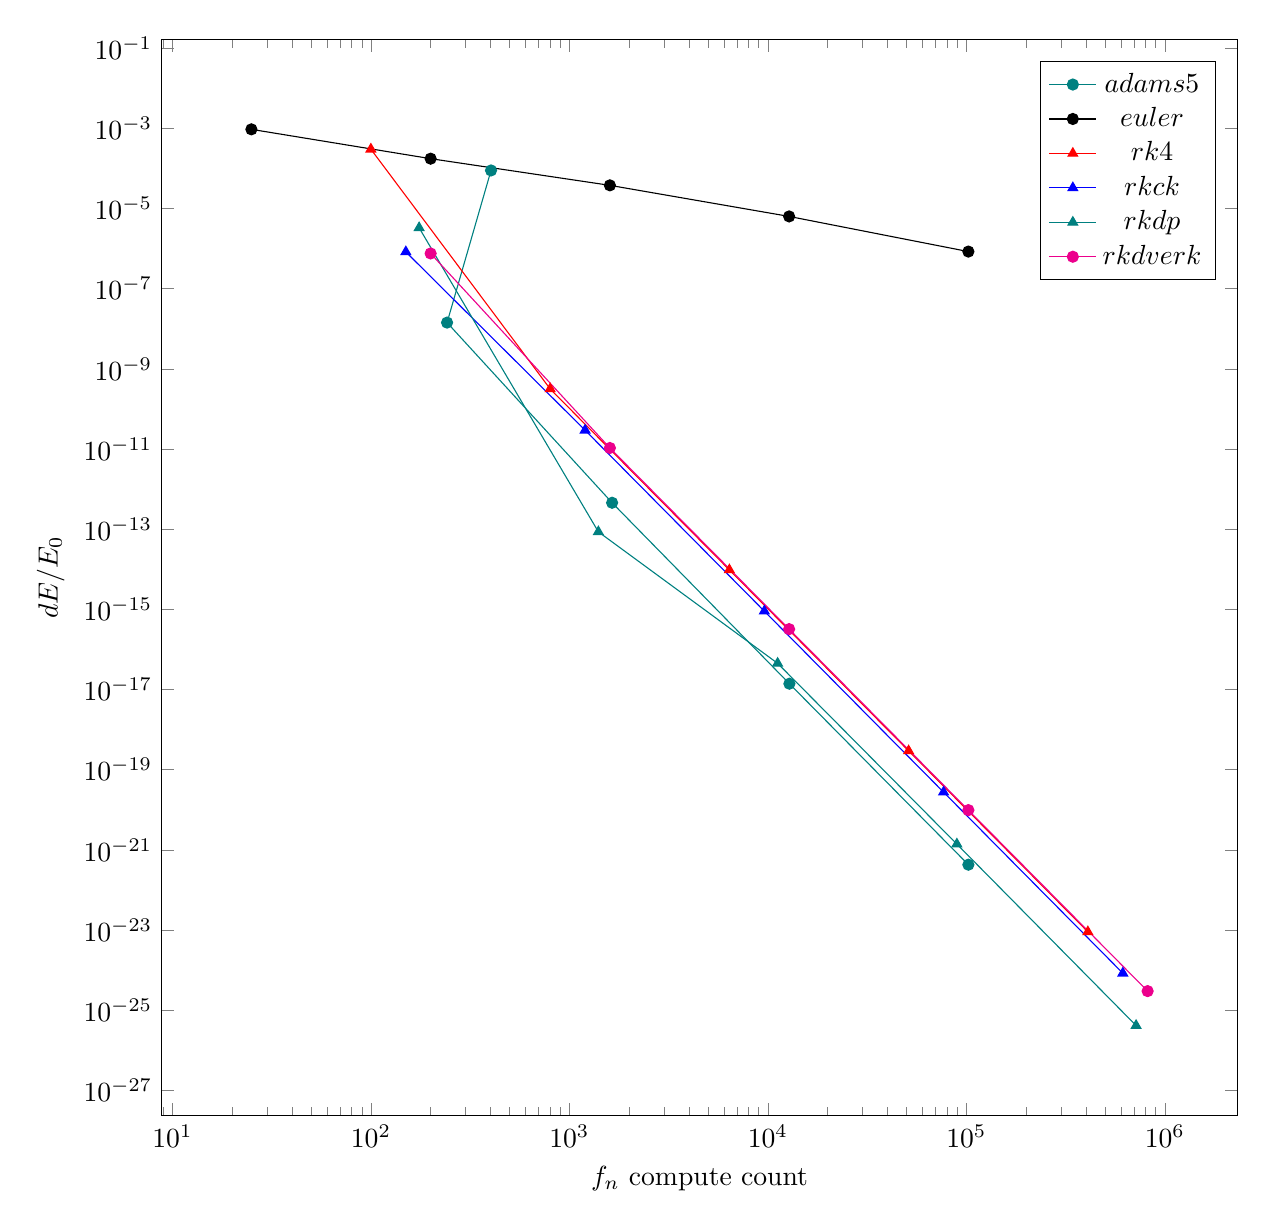
\begin{tikzpicture}
\begin{loglogaxis}[
    height=6in,
    width=6in,
    xlabel=$f_n$ compute count,
    ylabel=$dE/E_0$
]
\addplot [teal,mark=*,solid] coordinates { (403, 8.898e-05) (242, 1.424e-08) (1642, 4.556e-13) (1.284e+04, 1.395e-17) (1.024e+05, 4.26e-22) };
\addplot [black,mark=*,solid] coordinates { (25, 0.0009438) (200, 0.000175) (1600, 3.781e-05) (1.28e+04, 6.342e-06) (1.024e+05, 8.416e-07) };
\addplot [red,mark=triangle*,solid] coordinates { (100, 0.0003018) (800, 3.161e-10) (6400, 9.631e-15) (5.12e+04, 2.94e-19) (4.096e+05, 8.984e-24) };
\addplot [blue,mark=triangle*,solid] coordinates { (150, 8.278e-07) (1200, 2.944e-11) (9600, 9.007e-16) (7.68e+04, 2.748e-20) (6.144e+05, 8.374e-25) };
\addplot [teal,mark=triangle*,solid] coordinates { (175, 3.303e-06) (1400, 8.585e-14) (1.12e+04, 4.501e-17) (8.96e+04, 1.392e-21) (7.168e+05, 4.136e-26) };
\addplot [magenta,mark=*,solid] coordinates { (200, 7.555e-07) (1600, 1.061e-11) (1.28e+04, 3.211e-16) (1.024e+05, 9.796e-21) (8.192e+05, 2.99e-25) };
\legend{$adams5$,$euler$,$rk4$,$rkck$,$rkdp$,$rkdverk$};
\end{loglogaxis}
\end{tikzpicture}

\end{document}
